\clearpage

\lehead[]{\normalfont\sffamily\hspace*{-2.00cm}\textcolor{white}{\colorbox{lightblue}{\parbox[c][0.70cm][b]{1.60cm}{
\makebox[1.60cm][r]{\thechapter}\\ \makebox[1.60cm][r]{ÜBUNG}}}}\hspace{0.17cm}\textcolor{lightblue}{\chaptertitle}}
\rohead[]{\textcolor{lightblue}{\chaptertitle}\normalfont\sffamily\hspace*{0.17cm}\textcolor{white}{\colorbox{lightblue}{\parbox[c][0.70cm][b]{1.60cm}{\thechapter\\
ÜBUNG}}}\hspace{-2.00cm}}
%\chead[]{}
\rehead[]{\textcolor{lightblue}{AvHG, Inf, My}}
\lohead[]{\textcolor{lightblue}{AvHG, Inf, My}}

\section{Thread-Synchronisation -- Übungen}

\subsection{Aufgabe 1: Drucker-Simulation}

Fünf Threads teilen sich den Zugriff auf einen Drucker und müssen sich
untereinander abwechseln. Wir simulieren dies, in dem wir als \glqq
Drucker\grqq\ ein \myClass{JTextField} benutzen, in dem von den Threads
ein Text der Form \myUserInput{Thread 2 druckt \ldots} ausgegeben werden
soll.

Damit das Drucken in das Textfeld -- wie beim richtigen Drucken -- auch spürbar
Zeit verbraucht, kannst du die einzelnen Zeichen des Strings zeitlich verzögert
ausgeben lassen:

\begin{lstlisting}
for (int i = 0; i < zuDruckenderText.length(); i++) {
    drucker.tfDrucker.setText(drucker.tfDrucker.getText() + zuDruckenderText.charAt(i)); 
    try {
        Thread.sleep(300);
    } catch (InterruptedException e) {
        æ// Fehlerfall ignorieren
æ    }
}
\end{lstlisting}

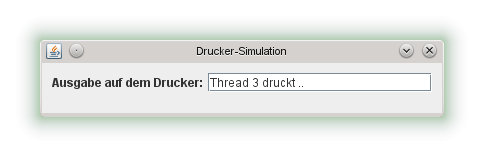
\includegraphics[width=0.7\textwidth]{./inf/SEKII/26_Java_Threads/Drucker-Simulation_synchronisiert.png}

Die Threads sollen in einer Endlosschleife immer abwechselnd drucken und
anschließend irgendwelche Berechnungen durchführen. Die Berechnung
soll durch einen \lstinline|sleep()|-Befehl, der eine
zufällig generierte Zeitspanne lang dauert, simuliert werden.
Erzeuge zur Simulation des Druckvorgangs Zufallszahlen zwischen 1 und 10  und
multipliziere das Ergebnis mit 150 Millisekunden.

Beachte, dass es in der Anwendung nur einen einzigen Zufallsgenerator geben
darf, den sich alle Threads teilen. Wenn jeder Thread seinen eigenen
Zufallsgenerator besitzt, erhalten alle Threads mit hoher Wahrscheinlichkeit
immer dieselben Zufallszahlen, weil alle Zufallsgeneratoren zur selben Zeit
gestartet werden.

Ohne geeignete Synchronisation werden sich die einzelnen Threads beim Drucken
ordentlich in die Quere kommen:

\begin{center}
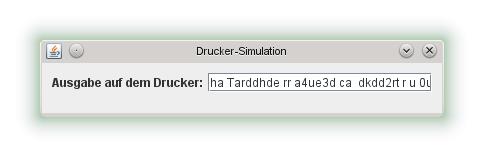
\includegraphics[width=0.7\textwidth]{./inf/SEKII/26_Java_Threads/Drucker-Simulation_nicht-synchronisiert.png}
\end{center}


\subsection{Aufgabe 2: Dining Philosophers}

Das berühmte Problem der {\em Dining Philosphers} wird häufig herangezogen um zu
illustrieren, was passieren kann, wenn mehrere Threads um dieselben Ressourcen
streiten.

\pagebreak

Die Geschichte lautet folgendermaßen:

\begin{quotation}
\noindent Fünf Philosophen sitzen um einen runden Tisch. Vor jedem Philosophen
steht eine Schüssel mit Reis. Zwischen je zwei Schüsseln liegt ein Stäbchen.
Damit ein Philosoph essen kann, benötigt er das Stäbchen links und rechts von
seiner Schüssel. Die Philosophen müssen sich so untereinander abstimmen, dass
alle abwechselnd essen können.
\end{quotation}

\begin{minipage}{0.6\textwidth}
\subsubsection{Überlegungen}

\begin{compactitem}
\item Wie viele Philosophen können maximal gleichzeitig essen?

\item Alle Philosophen arbeiten natürlich nach demselben Prinzip, damit man den
Code nur einmal programmieren muss. Was kann passieren wenn alle Philosophen
zuerst das Stäbchen an ihrer rechten Seite aufnehmen?
\end{compactitem}
\end{minipage}
\begin{minipage}{0.4\textwidth}
\begin{center}
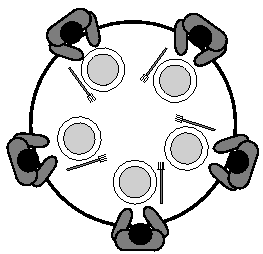
\includegraphics[width=0.5\textwidth]{./inf/SEKII/26_Java_Threads/Dining_Philosophers.png}
\end{center}
\end{minipage}

\subsubsection{Tipps für die Programmierung}

Programmiere eine Klasse \myClass{Philosoph}, die sich von der Superklasse
\myClass{Thread} ableitet. Erzeuge im Frame ein Array mit fünf Philosophen. Das
Frame enthält darüber hinaus ein Array mit den fünf Stäbchen (boolesche Werte,
die jeweils angeben, ob das betreffende Stäbchen genutzt wird oder nicht) und
ein Array mit den Philosophenbildern.

Die Bilder der Philosophen werden in der Frame-Methode
\lstinline|paintComponent()| gezeichnet. Jeder Philosophen-Thread hat eine
öffentliche Variable \lstinline|bildNr|, die die Nummer des aktuellen
Philosophen-Bildes angibt. Wenn sich die Nummer ändert, veranlasst der
Philosoph ein \lstinline|repaint()| des Frames.

Arbeitsweise eines Philosophen:

Die Philosophen rasten für eine zufällige Zeitspanne von 1 bis 5 mal 150
Millisekunden. Dann versuchen sie die Stäbchen zu ergreifen. Wenn sie beide
Stäbchen bekommen haben, starten sie mit dem Essen, andernfalls rasten sie
erneut für eine zufällige Zeitspanne und versuchen anschließend wieder die
Stäbchen zu ergattern. Das Essen ist ein längerer Zeitvorgang, der ebenfalls
zufällig gesteuert wird. Benutze hierzu \lstinline|Thread.sleep()| mit
zufälligen Wartezeiten von 1 bis 10 mal 150 Millisekunden. Nach dem Essen beginnen die
Philosophen wieder von vorne (Zuerst ruhen sie sich von dem anstrengenden Essen
aus, dann versuchen sie erneut die Stäbchen zu holen).

\begin{center}
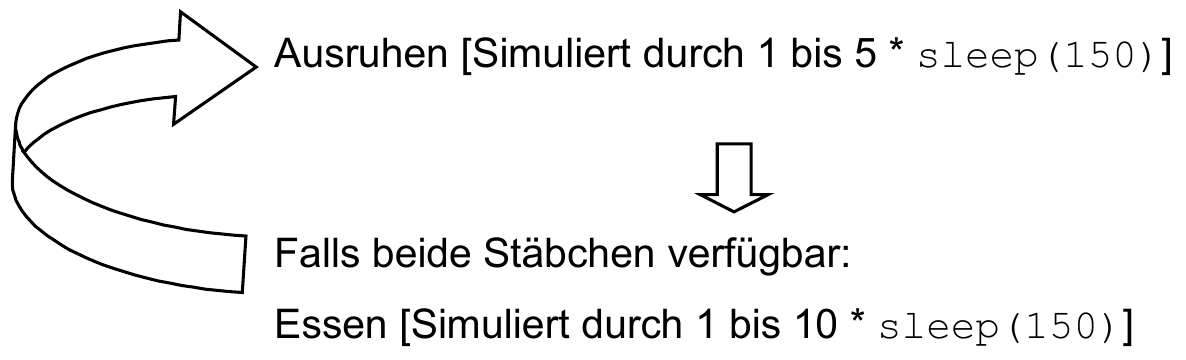
\includegraphics[width=0.6\textwidth]{./inf/SEKII/26_Java_Threads/Dining_Philosophers-Workflow.png}
\end{center}

\begin{center}
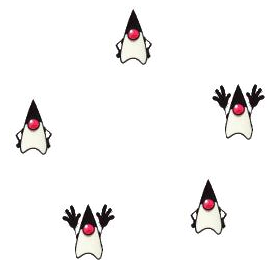
\includegraphics[width=0.4\textwidth]{./inf/SEKII/26_Java_Threads/Dining_Philosophers_Java.png}
\end{center}
